% ****** Start of file apssamp.tex ******
%
%   This file is part of the APS files in the REVTeX 4.1 distribution.
%   Version 4.1r of REVTeX, August 2010
%
%   Copyright (c) 2009, 2010 The American Physical Society.
%
%   See the REVTeX 4 README file for restrictions and more information.
%
% TeX'ing this file requires that you have AMS-LaTeX 2.0 installed
% as well as the rest of the prerequisites for REVTeX 4.1
%
% See the REVTeX 4 README file
% It also requires running BibTeX. The commands are as follows:
%
%  1)  latex apssamp.tex
%  2)  bibtex apssamp
%  3)  latex apssamp.tex
%  4)  latex apssamp.tex
%
\documentclass[%
 reprint,
%superscriptaddress,
%groupedaddress,
%unsortedaddress,
%runinaddress,
%frontmatterverbose, 
%preprint,
%showpacs,preprintnumbers,
%nofootinbib,
%nobibnotes,
%bibnotes,
 amsmath,amssymb,
 aps,
%pra,
%prb,
%rmp,
%prstab,
%prstper,
%floatfix,
]{revtex4-1}

\usepackage{graphicx}% Include figure files
\usepackage{dcolumn}% Align table columns on decimal point
\usepackage[spanish]{babel}
\selectlanguage{spanish} 
\usepackage[utf8]{inputenc}
\usepackage{bm}% bold math
%\usepackage{hyperref}% add hypertext capabilities
%\usepackage[mathlines]{lineno}% Enable numbering of text and display math
%\linenumbers\relax % Commence numbering lines
\usepackage{float}
%\usepackage[showframe,%Uncomment any one of the following lines to test 
%%scale=0.7, marginratio={1:1, 2:3}, ignoreall,% default settings
%%text={7in,10in},centering,
%%margin=1.5in,
%%total={6.5in,8.75in}, top=1.2in, left=0.9in, includefoot,
%%height=10in,a5paper,hmargin={3cm,0.8in},
%]{geometry}
\usepackage[font=footnotesize,labelfont=bf]{caption}
\usepackage{hyperref}
\newcommand{\subtitle}[1]{%
\posttitle{%
    \par\end{center}
\begin{center}\large#1\end{center}
\vskip0.5em}%
}
\begin{document}

%\preprint{APS/123-QED}

\title{Bombeo óptico\\ \textit{Estudio del efecto Zeeman fuerte y débil sobre un núcleo de Rubidio } }% Force line breaks with \\

%\subtitle{Estudio de la dualidad de onda partícula}

\author{Jose Alejandro Montaña Cortés}
\email{ja.montana@uniandes.edu.co}
% \altaffiliation[Also at ]{Departamento de Física, Universidad de los Andes}
\author{Jesús David Rincón Puche}%
\email{jd.rincon883@uniandes.edu.co}
\affiliation{Departamento de Física, Universidad de los Andes}%

%\collaboration{}%\noaffiliation

\date{\today}% It is always \today, today,
             %  but any date may be explicitly specified

\begin{abstract}



\end{abstract}
\maketitle
%\tableofcontents

%---------------------INTRODUCCIÓN------------------
\section{Introducción}
 El entendimiento de las propiedades cuánticas de los átomos, tales como los números cuánticos que caracterizan el momento angular de un núcleo atómico, resultan ser una parte fundamental de mecánica cuántica, pues estas propiedades determinan el comportamiento de los espectros y por ende proporcionan una forma de caracterizar los distintos elementos. El bombeo óptico, permite excitar electrones de los núcleos a distintos estados. En esta práctica se muestra como estados que aparentan ser degenerados, pueden ser separados gracias a la interacción del átomo con un campo magnético. Particularmente se toman núcleos de Rubidio (Rb) y se ponen a interactuar con un campo magnético. Debido a el efecto Zeeman, a medida que el campo magnético externo se incrementa, la separación entre los niveles se hace más notoria, lo cual permite su observación en un montaje experimental relativamente simple.
 Debido a las reglas de selección de la mecánica cuántica, existen un conjunto posibles de transiciones permitidas a las cuales electrones pueden acceder. Basado en esto y la intensidad de campo magnético aplicado, es posible determinar que tan grande será la separación entre los niveles que eran previamente degenerados.
 \section{Marco Teórico}
 
 
% trim={<left> <lower> <right> <upper>}
%----MONTAJE EXPERIMENTAL--------
\section{Montaje experimental}
\subsection{Instrumento de medición.}
Para este experimento se hizo uso del aparato de ``optical pumping'' de la marca TechSpin. Este aparato cuanta con una lampara de descarga RF (Radio frequency), un filtro de interferencia, un polarizador lineal, un polarizador de cuarto de onda, una cámara con rubidio\footnote{El vapor cámara de absorción del rubidio está encerrada en un horno de plexiglass, el cual permitía controlar la temperatura y por ende la presión de vapor del rubidio.}, 2 lentes focalizadores y un detector óptico, tal configuración puede observarse en la figura \ref{montaje experimental}
\begin{figure}[h]
\center{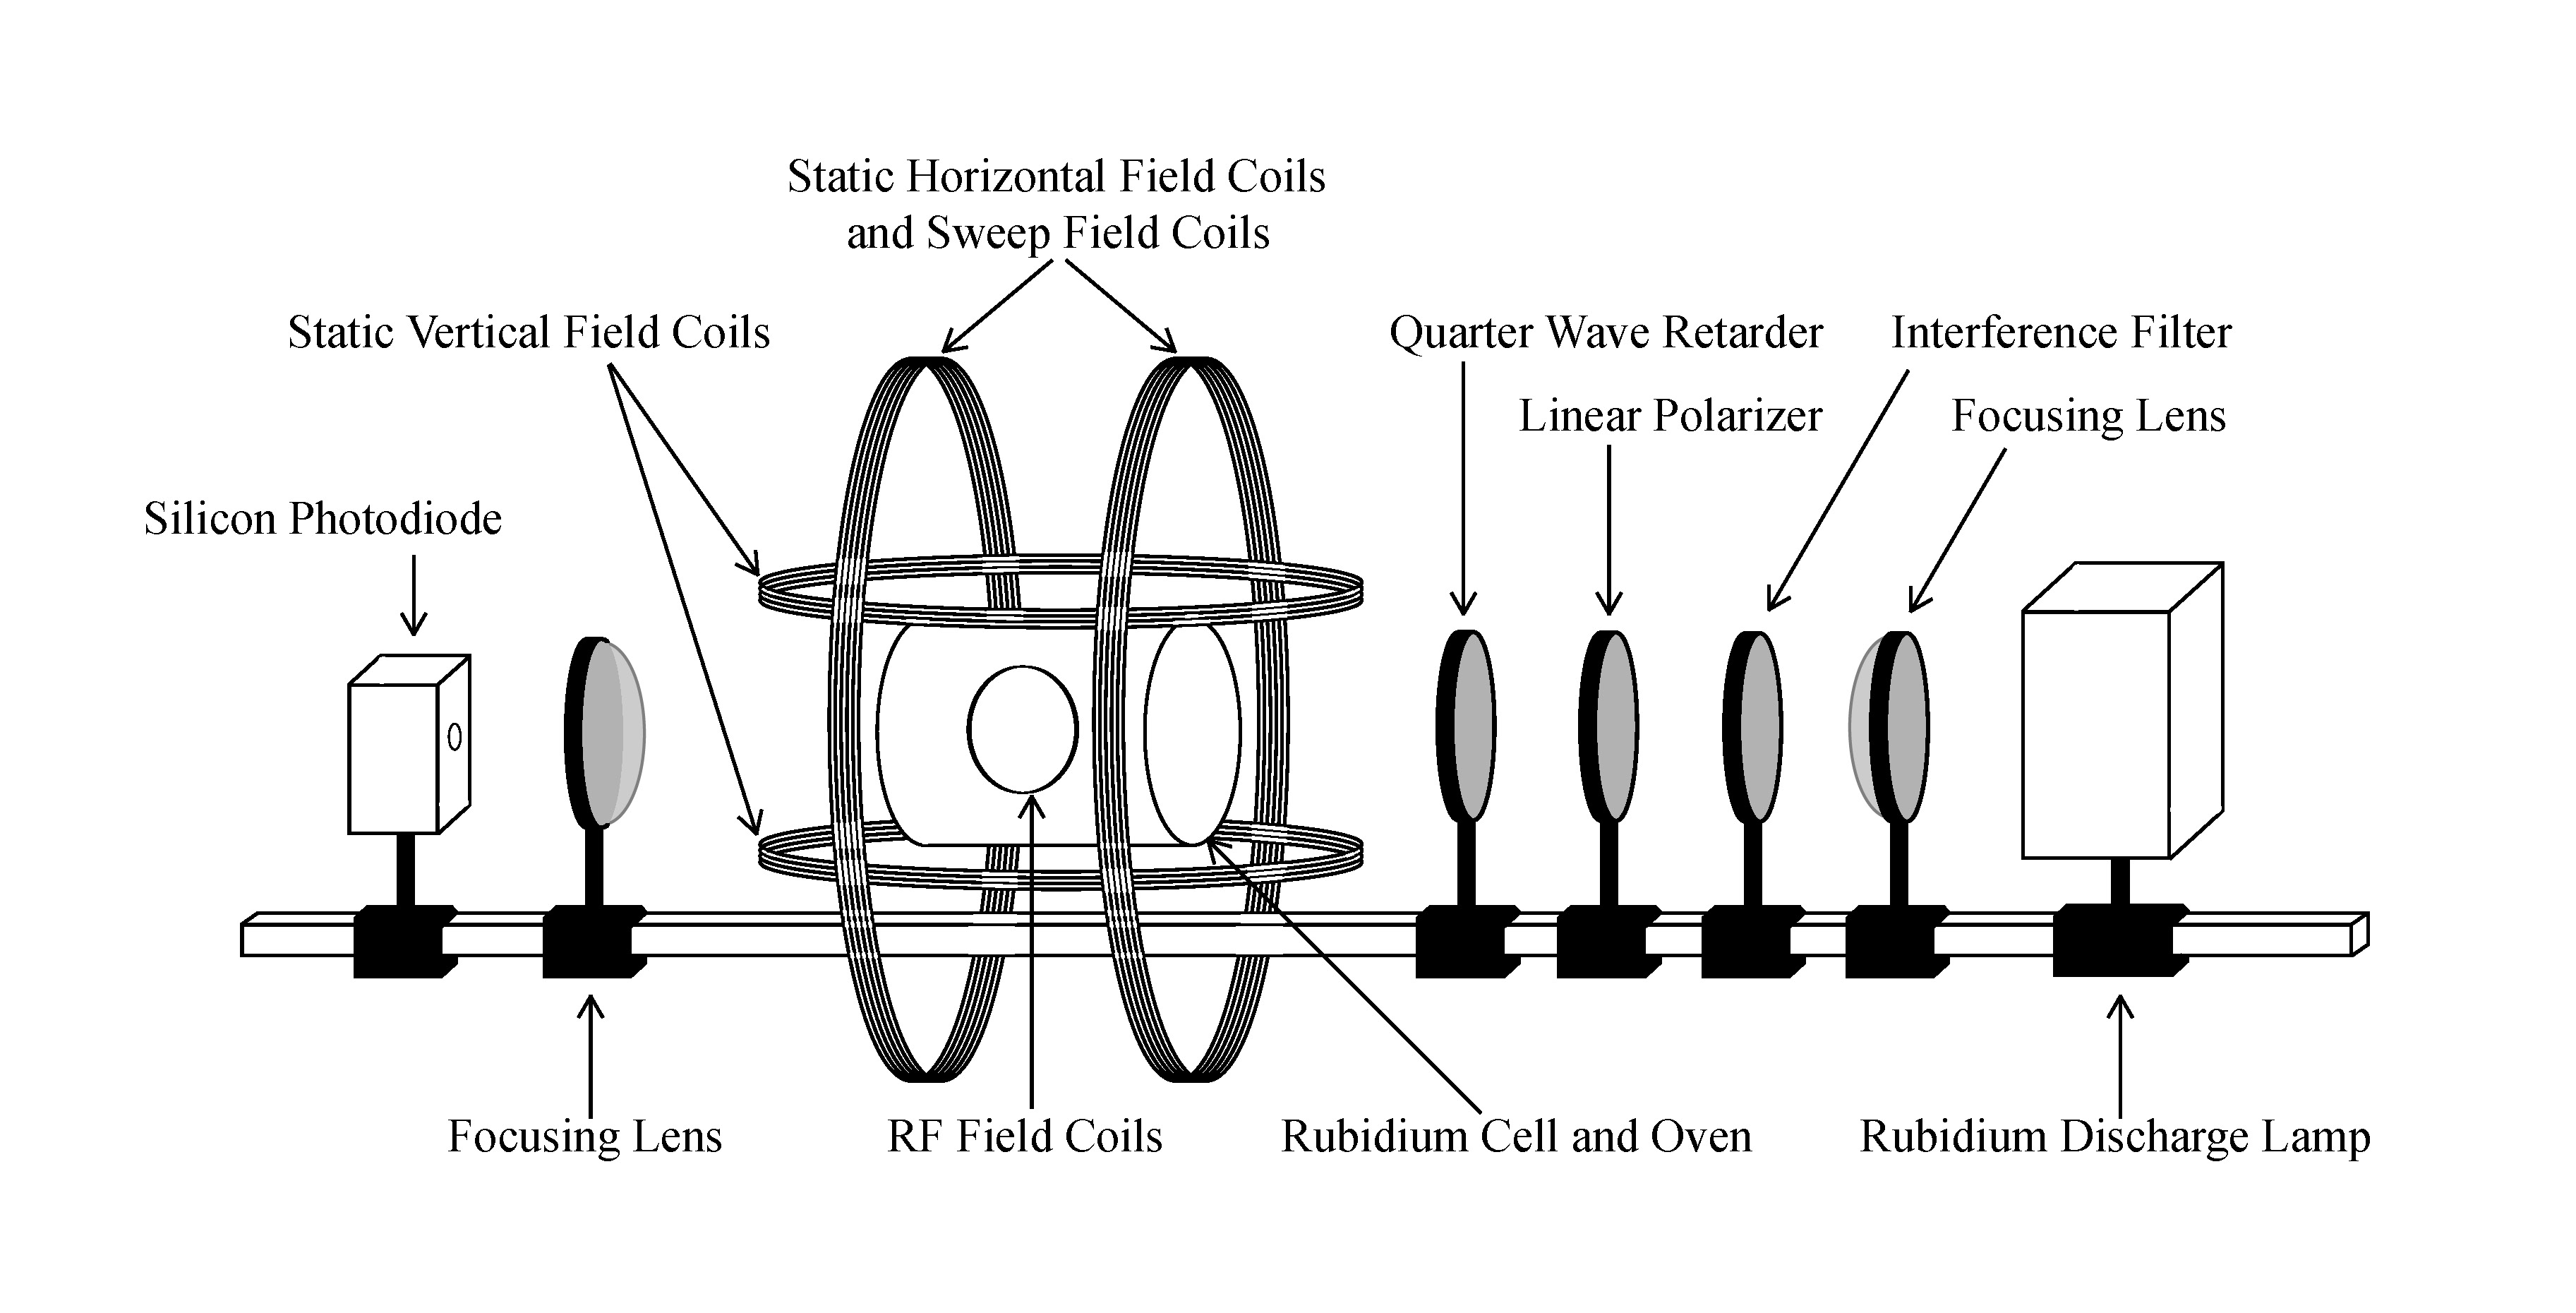
\includegraphics[width=0.4\textwidth]
{../Figuras/apparatus.jpg}}
\caption{\label{montaje experimental} Esquema del montaje experimental usado en este experimento.  (tomado de \cite{figura_aparato}).}
\end{figure}
La cámara en donde se encontraba el Rubidio estaba rodeada por 2 bobinas de Helmholtz para así producir los campos magnéticos. Uno de estos campos debe estar alineado con el campo magnético terrestre, configuración que se obtuvo haciendo uso de una brújula, esto con el fin de que el campo generado por las bobinas Helholtz contrarrestara el campo terrestre y así de esta forma calibrar nuestras mediciones. el otro conjunto de bobinas de Helmholtz es usado para crear un campo magnético de ``barrido'', el cual nos permite identificar la intensidad de los campos magnéticos en los cuales las transiciones ocurren.\\
El cable de RF es el encargado de revertir algunos de los efectos en el bombeo de los isótopos del Rb. Esto se logra al ajustar esta frecuencia en los estados que están siendo excitados.Para el caso del estado base, también se tiene que los fotones pueden ser absorbidos y por ende se observará una caída en la intensidad del detector.
\subsection{Configurando el aparato}
Con el fin de lograr visualizar los niveles de energía del rubidio se tuvo que calibrar inicialmente el montaje, esto con la finalidad de lograr que se asegurara una polarización circular de la luz, se puso el polarizador de media onda a un ángulo de 39 grados y con el fin de verificar que si se tenía polarización circular se dispuso un polarizador lineal al frente de la configuración (polarizador lineal y el de media onda) y se veía si la intensidad en el detector variaba al cambiar la disposición del último polarizador lineal, al no haber observado cambio significativo en el detector, se concluyo que se estaba trabajando con polarización circular tal y como se requería. Seguido a esto se procedió a ajustar el campo magnético vertical en $0.1A$ y se fijó la ganancia en 200, luego se empezó a cambiar el valor del campo magnético de barrido para encontrar el valor de campo que producía el pico de transición que se buscaba. Una vez encontrada esta configuración se procedió a conectar el generador RF y se hizo un estudio del efecto de la radio frecuencia en función de la corriente a la cual se encontraban los picos. Por último se puso un generador de onda cuadrada y se ubicó uno de los picos anteriormente encontrados, la onda generada era de tipo cuadrada y y se dispuso un voltaje de $10V$ de pico a pico a una frecuencia de $5Hz$, esto con el fin de analizar los periodos generados en las oscilaciones de Rabi para cada uno de los picos, en esta parte se varió la intensidad de la radio frecuencia de entrada.\\
A continuación se muestran los resultados obtenidos.


%-----------------RESULTADOS----------------------
\section{Resultados y Análisis}


%---------------CONCLUSIONES-------------------

\section{Conclusiones}
\begin{itemize}
    \item 
\end{itemize}
%Se deben contestar las preguntas planteadas inicialmente o dar las razones por las cuales no es posible hacerlo. Las conclusiones deben ser necesariamente una consecuencia del experimento realizado, es decir que no se deben tocar aspectos que no se hayan expuesto en la sección de resultados y análisis. Si escribe algo que no se encuentra en la sección de resultados y análisis, esto quiere decir que hace falta incluir material en resultados y análisis. Concluir únicamente aspectos pertinentes a su trabajo en el laboratorio; evite generalizaciones que no hablan concretamente de lo que usted hizo o midió.

\begin{thebibliography}{9}
\bibitem{figura_aparato}
\url{http://spa-mxpweb.spa.umn.edu/s11/Projects/S11_OpticalPumping/apparatus.htm}

\end{thebibliography}

\end{document}
%
% ****** End of file apssamp.tex ******

